%-------------------------------------------------------------------------------------------------%
% Author: John Joseph Valletta
% Date: 08/02/2015
% Title: Introduction to Machine Learning for the Life Sciences
%-------------------------------------------------------------------------------------------------%
% Preamble
\documentclass[pdf]{beamer}
\usepackage{textpos} % for logo placement in headline
\usepackage[export]{adjustbox}
\newif\ifplacelogo % Create a new conditional to avoid displaying logo on every slide
\placelogotrue % Set it to true
\mode<presentation>{\usetheme{Madrid}} % default Antibes Berlin Madrid Montpelier Ilmenau CambridgeUS Berkeley Singapore Copenhagen Malmoe Warsaw
\usecolortheme{dolphin}
\useinnertheme{circles} % circles, rectanges, rounded, inmargin
%\useoutertheme{tree} % infolines, smoothbars, sidebar, split, tree
\setbeamercovered{transparent=5} % Transparent 10% overlays
\setbeamertemplate{caption}{\raggedright\insertcaption\par} % Remove the word "Figure" from caption %\setbeamertemplate{caption}[default]
\setbeamertemplate{navigation symbols}{} % don't put navigation tools at the bottom (alternatively \beamertemplatenavigationsymbolsempty)
\graphicspath{ {./Figures/} }

% Titlepage
\title{Introduction to Machine Learning}
\subtitle{for the Life Sciences}
\author{JJ Valletta}
% Logo
\logo{\ifplacelogo
\includegraphics[width=4cm,keepaspectratio, left]{logo2.pdf}\fi}
\addtobeamertemplate{headline}{}{\ifplacelogo
\begin{textblock*}{100mm}(.68\textwidth,+0.1cm)%.015 instead of 0.68 originally

\includegraphics[width=4cm,keepaspectratio]{logo1.pdf}
\end{textblock*}\fi}
%\author{John Joseph Valletta, Alex Thornton and Mario Recker}
%-------------------------------------------------------------------------------------------------%
% Start of Document
%-------------------------------------------------------------------------------------------------%
\begin{document}
%-------------------------------------------------------------------------------------------------%
% Slide 0: Title Slide
\begin{frame}
\titlepage
\end{frame}
%-------------------------------------------------------------------------------------------------%
\begin{frame}{Housekeeping}
\begin{itemize}
	\item Who are we?
	\item Timetable
	\item Important Info
	\item Contact emails
\end{itemize}
\end{frame}
%-------------------------------------------------------------------------------------------------%
\begin{frame}{Workshop learning outcomes}
\begin{itemize}\addtolength{\itemsep}{0.5\baselineskip}
	\item Understand the key concepts and terminology used in the field of machine learning
	\item Apply machine learning algorithms in R and apply them to your own datasets
	\item Recognise practical issues in data analysis
\end{itemize}
\end{frame}
\placelogofalse % Turn logo off
%-------------------------------------------------------------------------------------------------%
\begin{frame}{Overview}
\begin{itemize}\addtolength{\itemsep}{0.5\baselineskip}
	\item<2-> What is machine learning?
	\item<3-> Types of learning methods
	\item<4-> Statistics vs Machine Learning
	\item<5-> Formulating a machine learning problem
	\item<6-> Terminology
	\item<7-> Applications in life sciences
\end{itemize}
\end{frame}
%-------------------------------------------------------------------------------------------------%
\begin{frame}{What my mum thinks machine learning is}
\begin{center}
	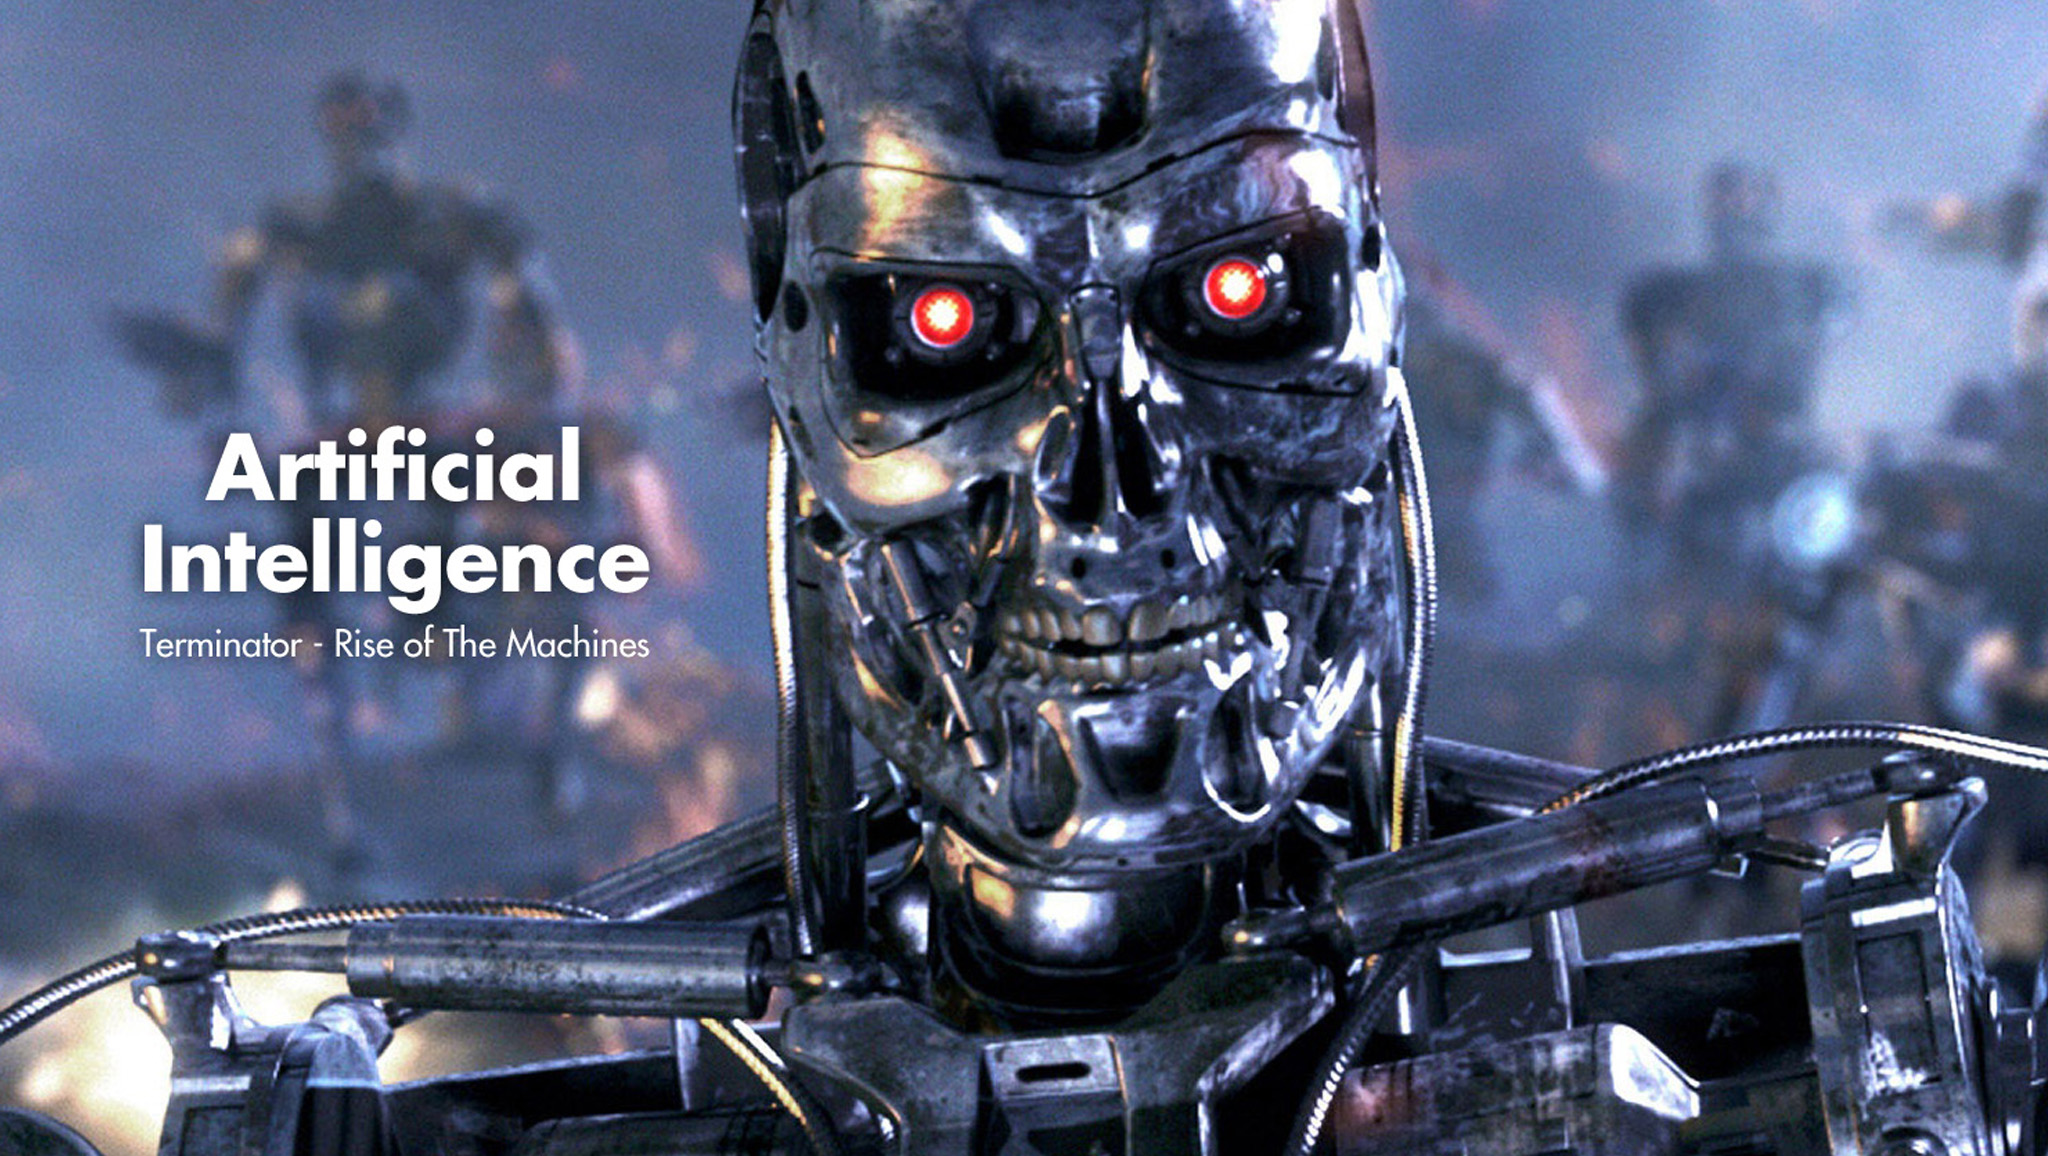
\includegraphics[width=\textwidth]{AI.jpg}
\end{center}
\end{frame}
%-------------------------------------------------------------------------------------------------%
\begin{frame}{Who uses machine learning?}
\begin{columns}
\column{0.33\textwidth}
\begin{center}
	
\includegraphics[width=\textwidth]{google.png}
	\vspace{2cm}
	
\includegraphics[width=0.5\textwidth]{facebook.png}
\end{center}
\column{0.33\textwidth}
\begin{center}
	
\includegraphics[width=\textwidth]{netflix.png}\\
	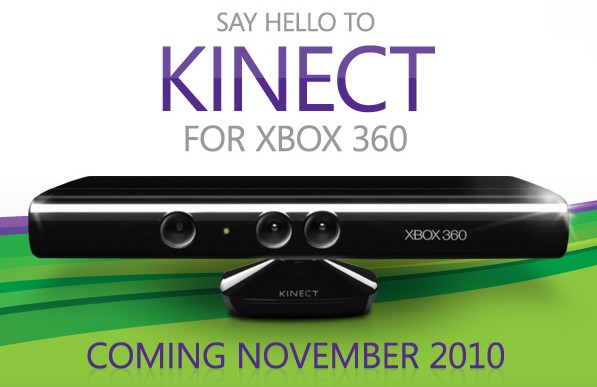
\includegraphics[width=\textwidth]{kinect.jpg}\\
	
\includegraphics[width=\textwidth]{youtube.png}
\end{center}
\column{0.33\textwidth}
\begin{center}
	
\includegraphics[width=0.5\textwidth]{AXA.png}\\
	\vspace{2cm}
	
\includegraphics[width=\textwidth]{amazon.jpg}
\end{center}
\end{columns}
\end{frame}
%-------------------------------------------------------------------------------------------------%
\begin{frame}{Who uses machine learning?}
\begin{columns}
\column{0.55\textwidth}
\begin{center}
	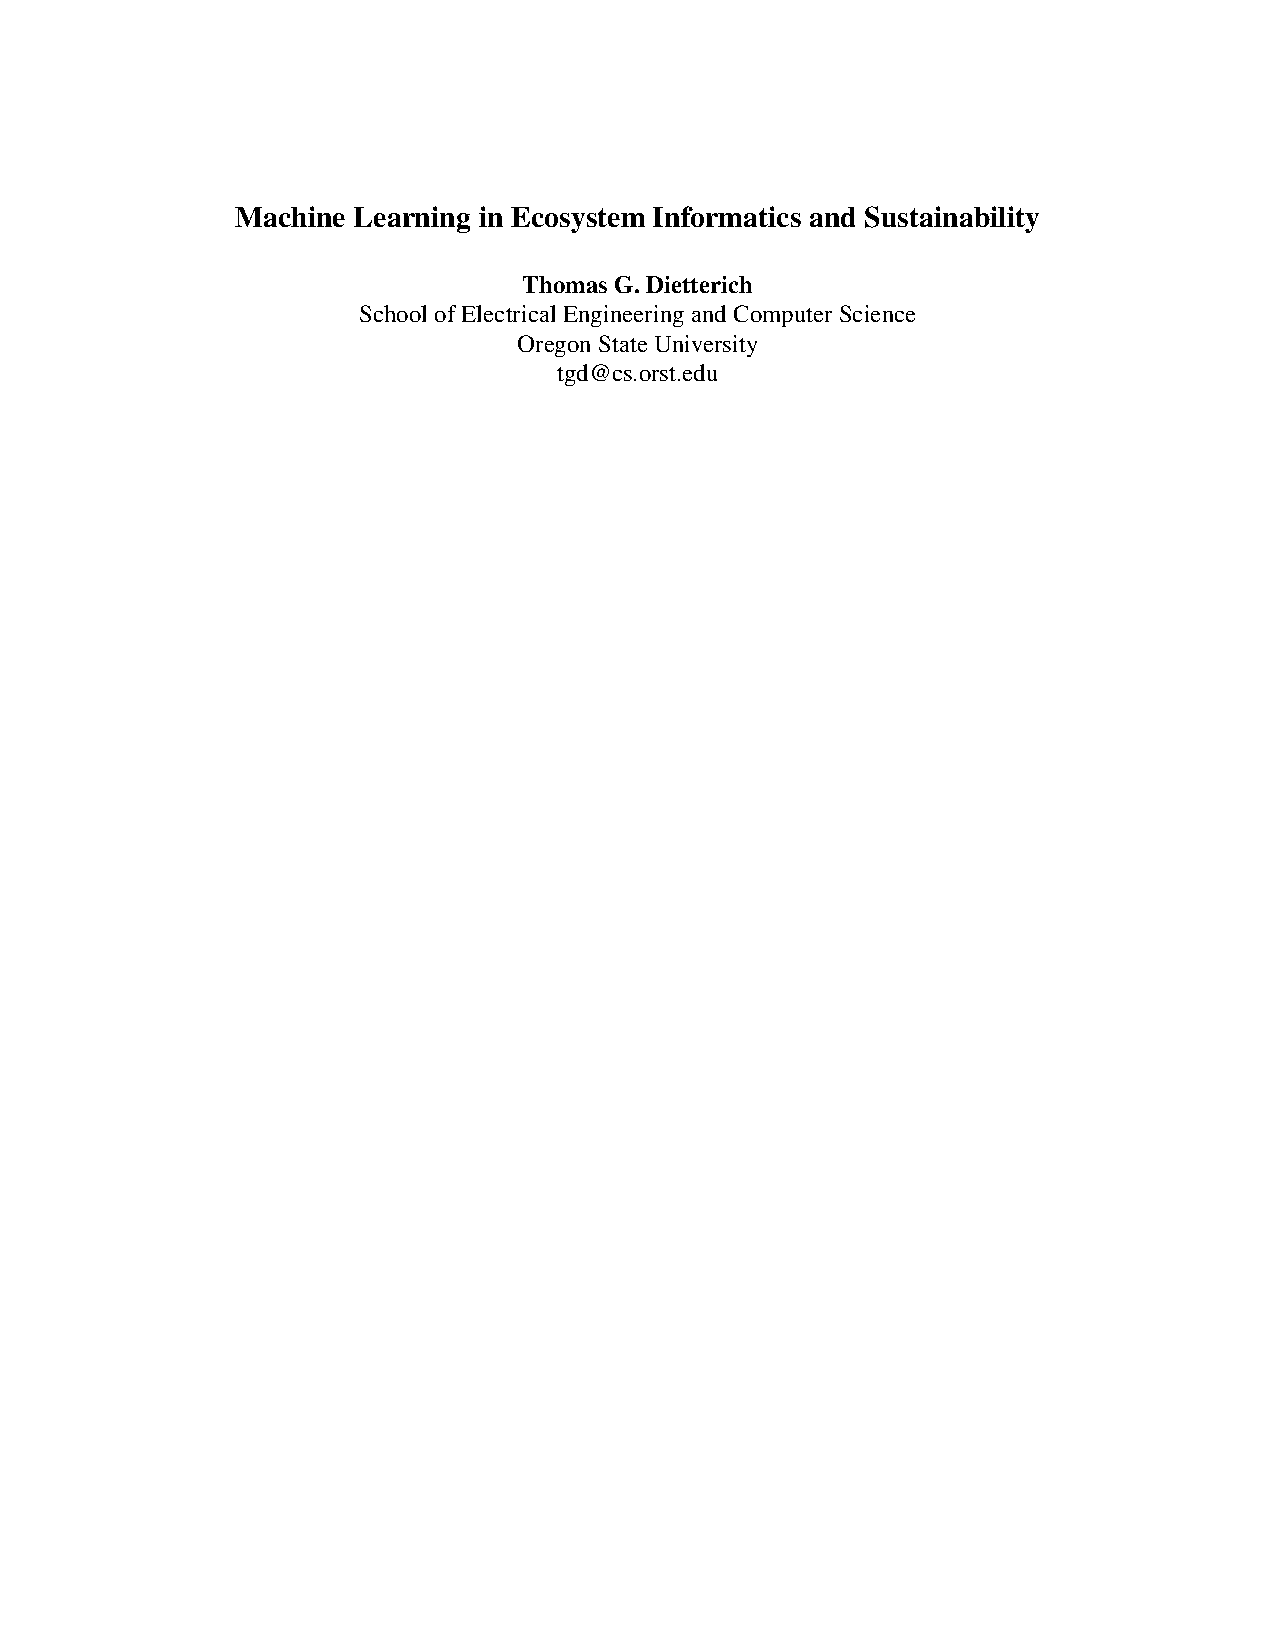
\includegraphics[width=\textwidth]{useML01.pdf}\\
	\vspace{2cm}
	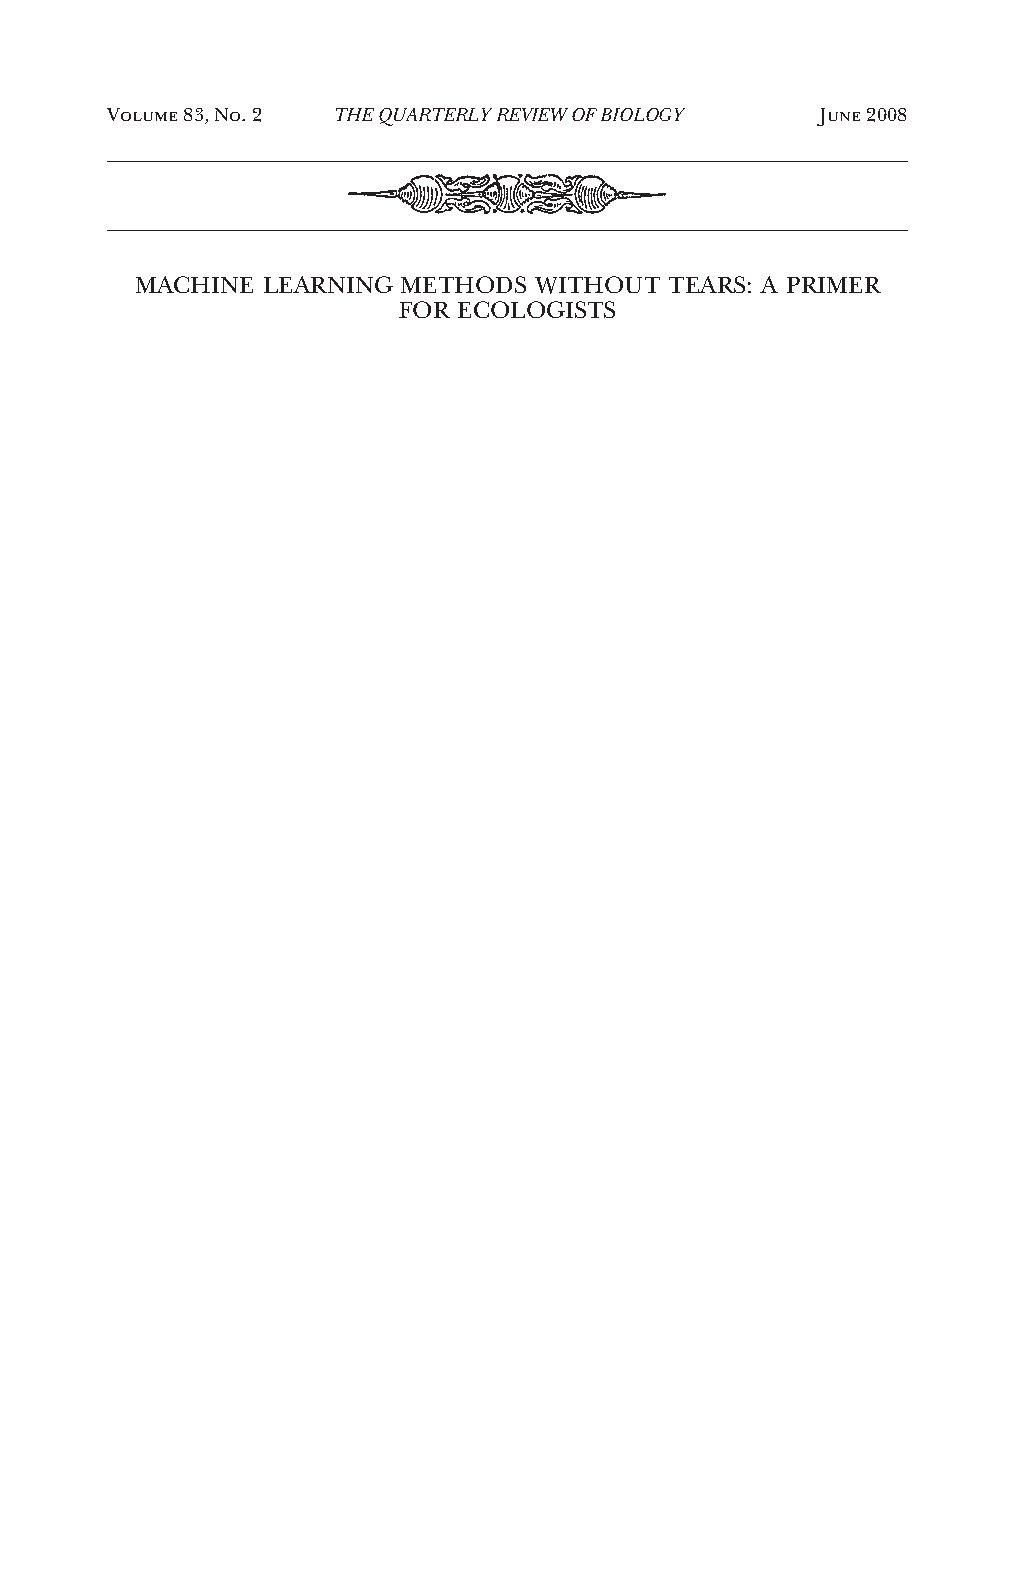
\includegraphics[width=\textwidth]{useML02.pdf}
\end{center}
\column{0.45\textwidth}
\begin{center}
	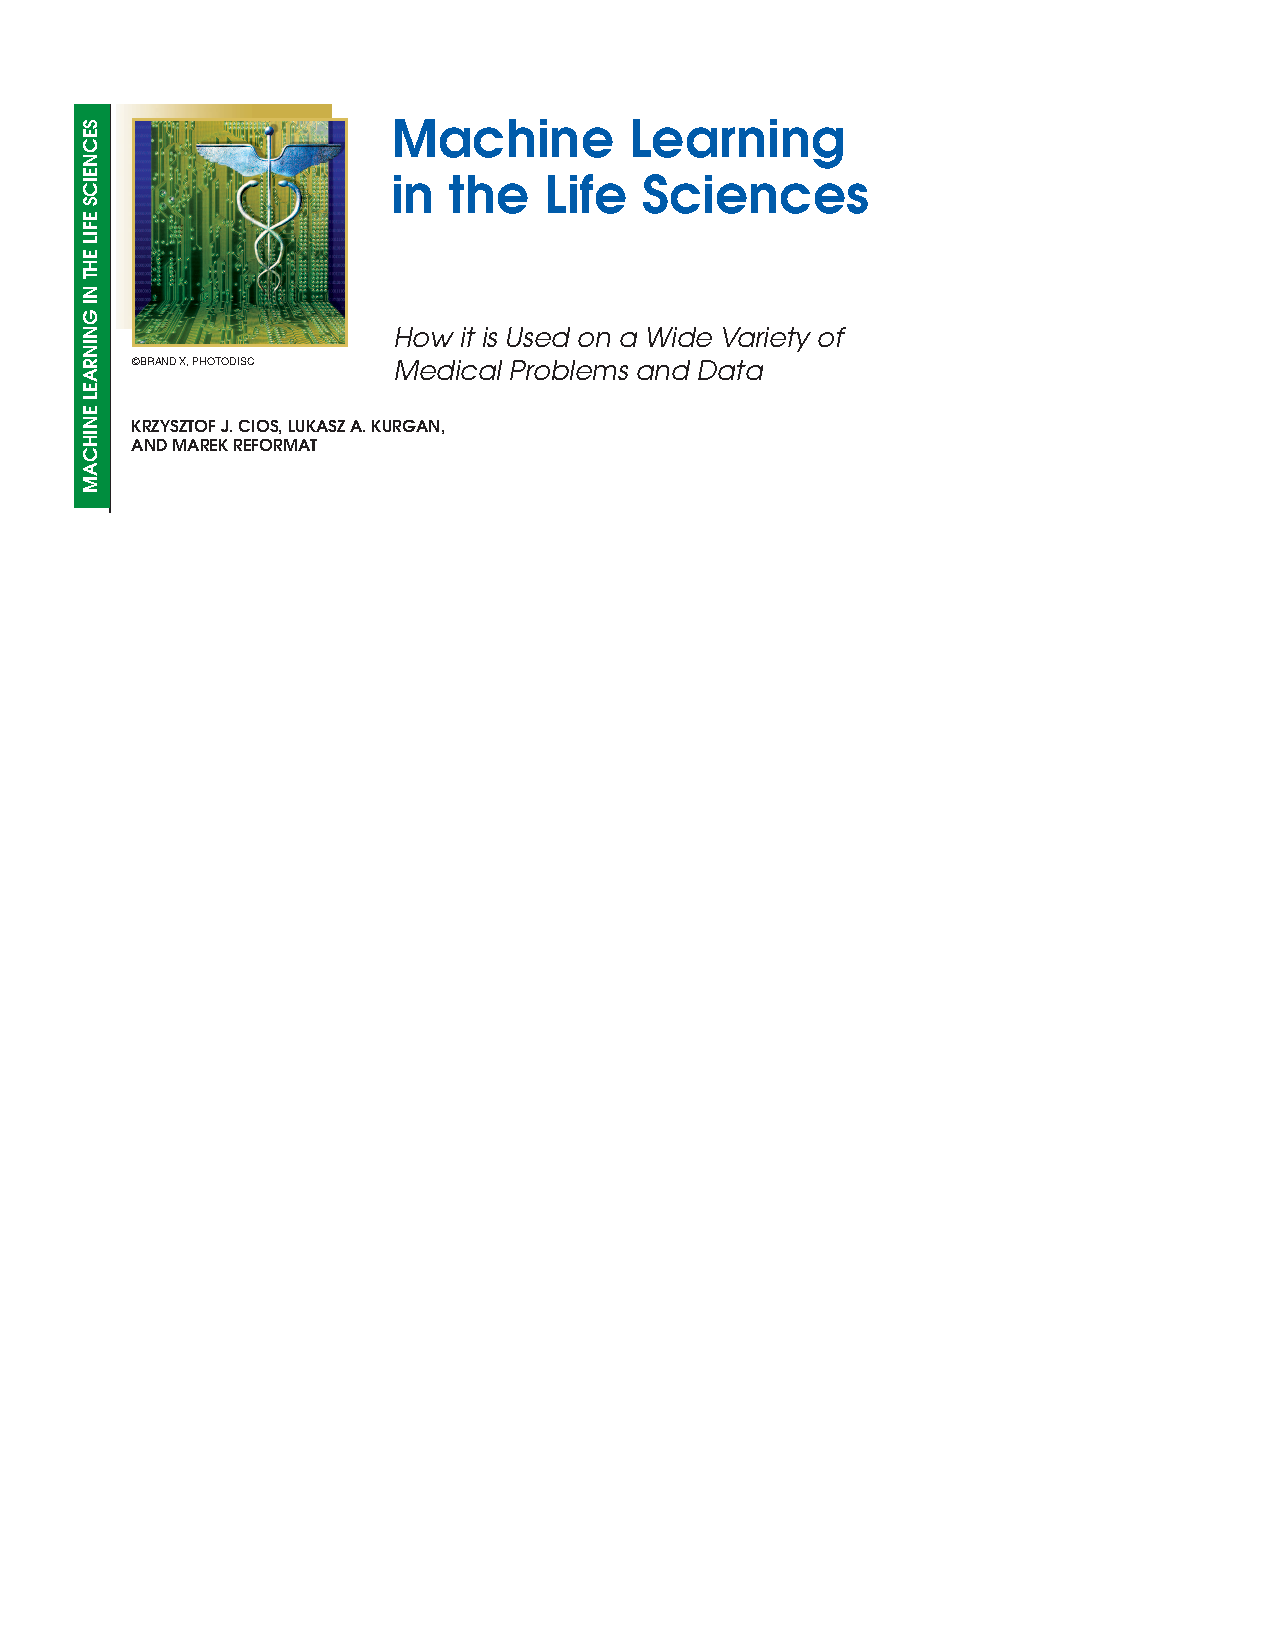
\includegraphics[width=\textwidth]{useML03.pdf}\\
	\vspace{2cm}
	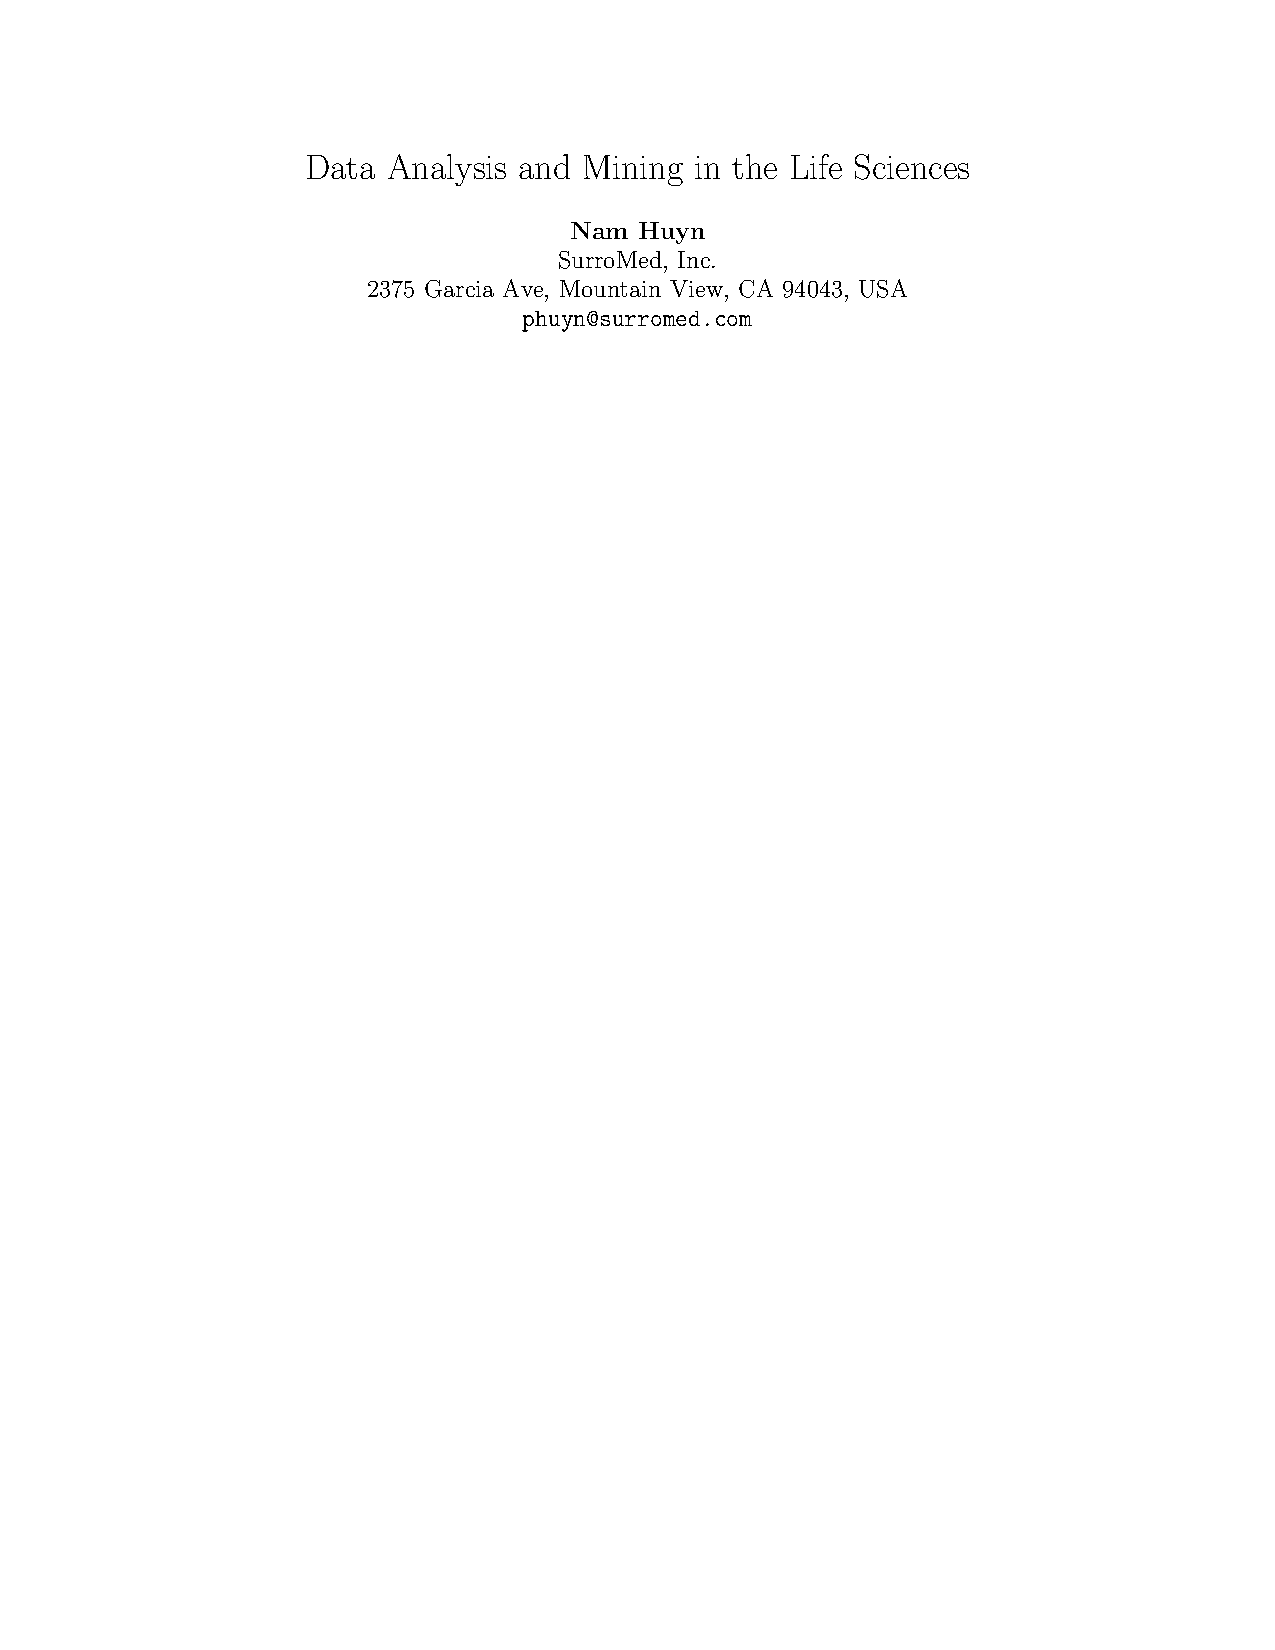
\includegraphics[width=\textwidth]{useML04.pdf}
\end{center}
\end{columns}
\end{frame}
%-------------------------------------------------------------------------------------------------%
\begin{frame}{There are even competitions now!}
\begin{center}
	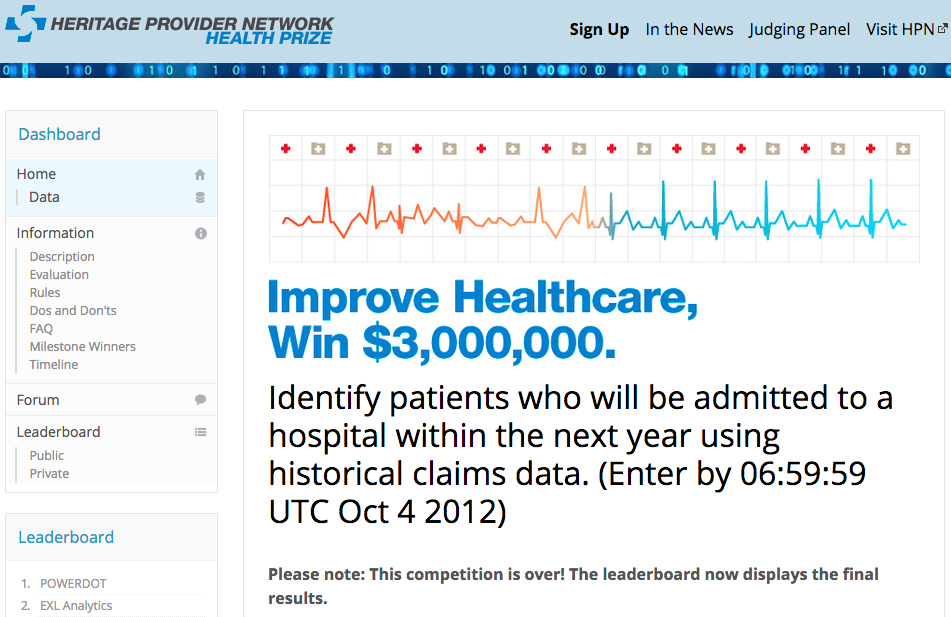
\includegraphics[width=\textwidth]{competition.png}
\end{center}
\end{frame}
%-------------------------------------------------------------------------------------------------%
\begin{frame}{Lots of them actually...}
\begin{figure}
\begin{center}
	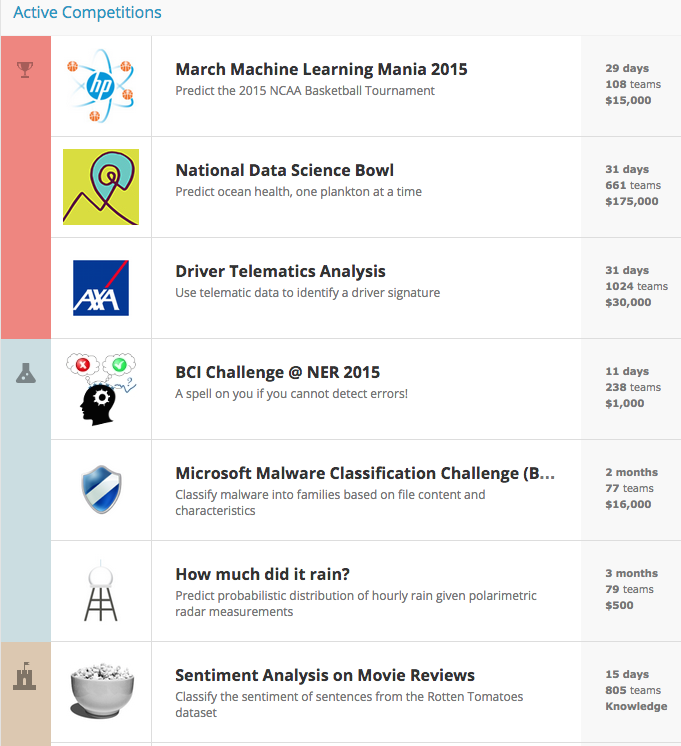
\includegraphics[width=0.55\textwidth]{competitions.png}
	\caption{\small{Source: http://www.kaggle.com/}}
\end{center}
\end{figure}
\end{frame}
%-------------------------------------------------------------------------------------------------%
\begin{frame}{So what is machine learning?}
\visible<2->{\begin{exampleblock}{}
{\small A machine learns with respect to a particular
task T, performance metric P, and type of experience E, if the system reliably improves its performance
P at task T, following experience E }
\vskip5mm
\hspace*\fill{\footnotesize --- Tom Mitchell}
\end{exampleblock}}
\vfill
\visible<3->{\begin{exampleblock}{}
{\small A scientific discipline that explores the construction and study of algorithms that can learn from data. 
Such algorithms operate by building a model from example inputs and using that to make predictions or decisions, 
rather than following strictly static program instructions.}
\vskip5mm
\hspace*\fill{\footnotesize --- Wikipedia}
\end{exampleblock}}
\vfill
\visible<4->{\begin{exampleblock}{}
{\small Machines learn using flashcards}
\vskip5mm
\hspace*\fill{\footnotesize --- JJ}
\end{exampleblock}}
\end{frame}
%-------------------------------------------------------------------------------------------------%
\begin{frame}{Group by shape (unsupervised learning)}
\begin{center}
	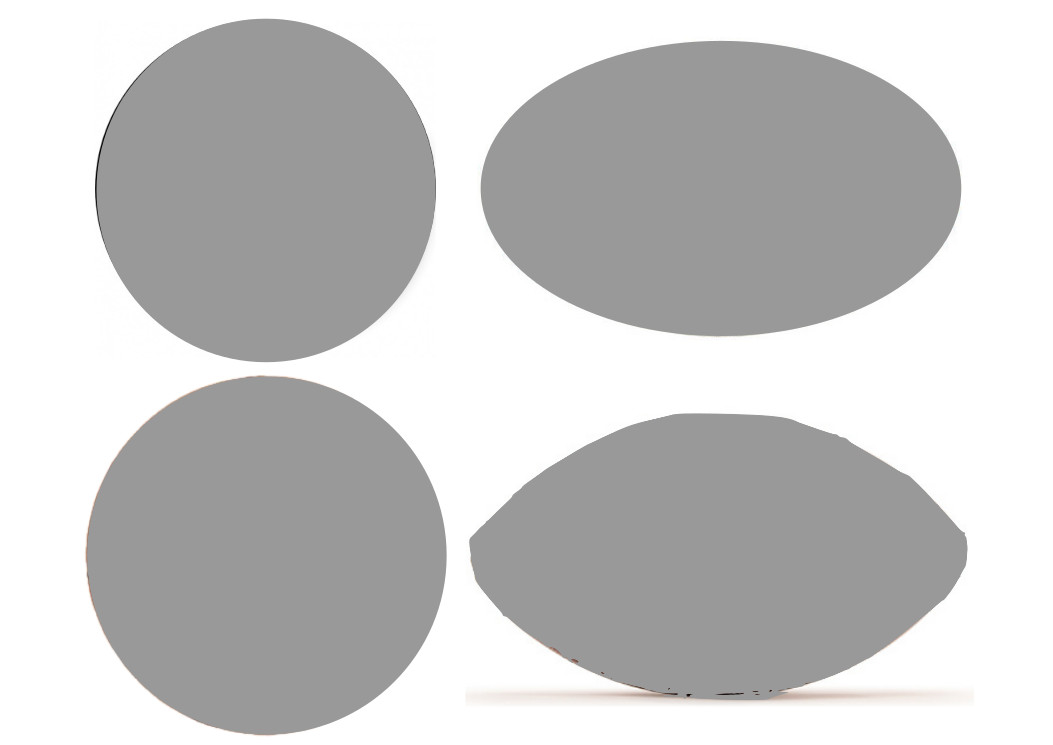
\includegraphics[width=0.9\textwidth]{flashcardHidden.png}
\end{center}
\end{frame}
%-------------------------------------------------------------------------------------------------%
\begin{frame}{Add labels (supervised learning)}
\begin{center}
	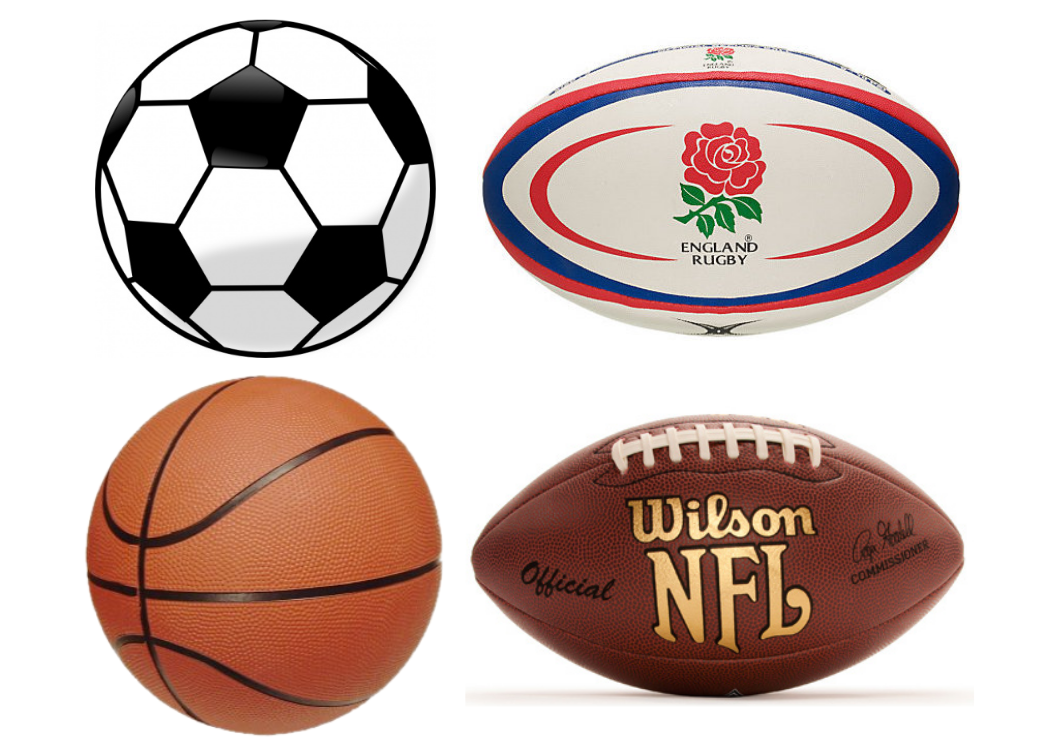
\includegraphics[width=0.9\textwidth]{flashcardExposed.png}
\end{center}
\end{frame}
%-------------------------------------------------------------------------------------------------%
\begin{frame}{Types of learning methods}
\small
\begin{description}[Reinforcement learning:]
	\item<2->[Unsupervised learning:] Inputs have \textit{no} corresponding output labels
		\begin{itemize}
			\item \textbf{Clustering} - discovering groups having similar attributes (e.g unlabelled gene expression profiles)
			\item \textbf{Density Estimation} - determine probability distribution of data (e.g species distribution model)
			\item \textbf{Dimensionality Reduction} - identify and remove redundant dimensions 
		\end{itemize}
	\item<3->[Supervised learning:] Inputs have corresponding output labels
		\begin{itemize}
			\item \textbf{Regression} - output is a continuous variable (e.g $CO_2\ concentration\ ppm$ )
			\item \textbf{Classification} - output is categorical (e.g benign (0) or cancerous (1) tumour)
		\end{itemize}	
	\item<4->[Reinforcement learning:] Finding suitable actions to maximise a reward by a
	process of trial and error. Tradeoff between exploration (use new actions) vs exploitation
	(use actions already known to work) 
\end{description}
\end{frame}
\normalsize
%-------------------------------------------------------------------------------------------------%
\begin{frame}{Statistics vs Machine Learning}
\begin{center}
	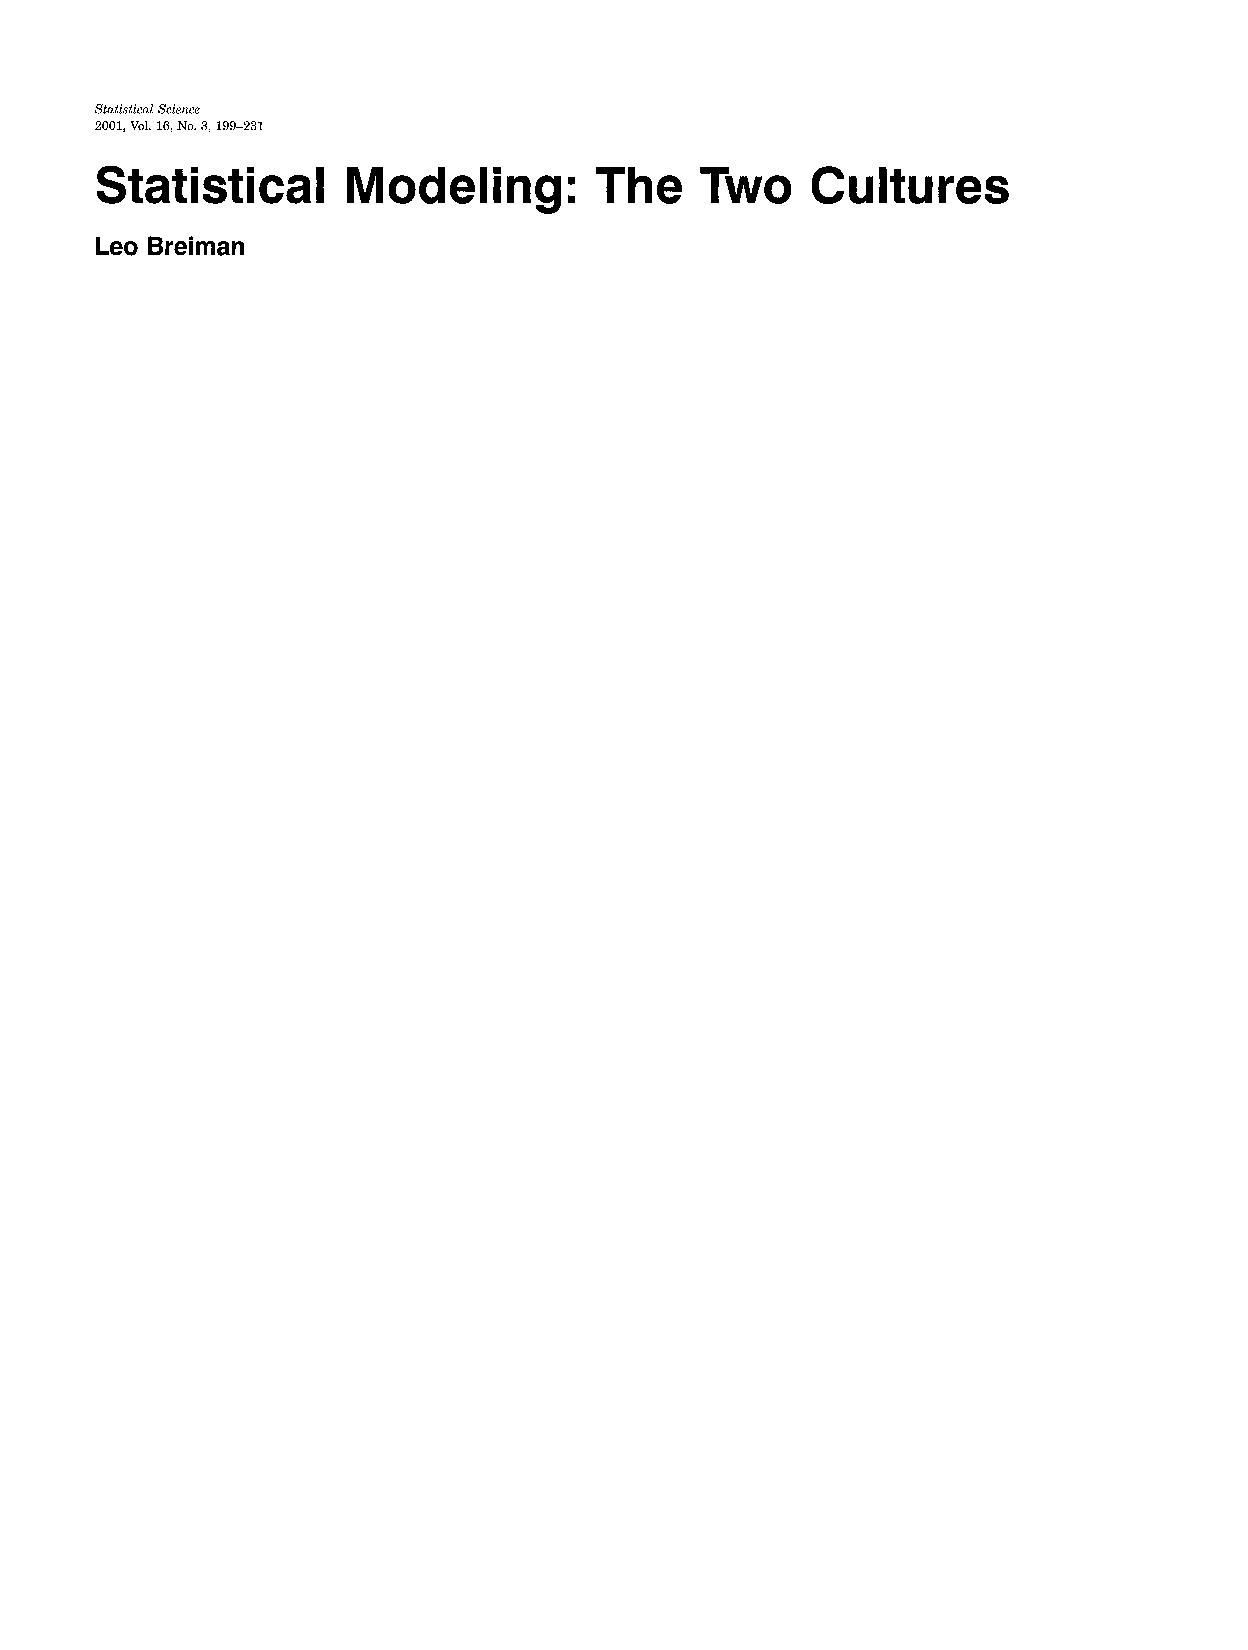
\includegraphics[width=\textwidth]{breimanPaper.pdf}\\
	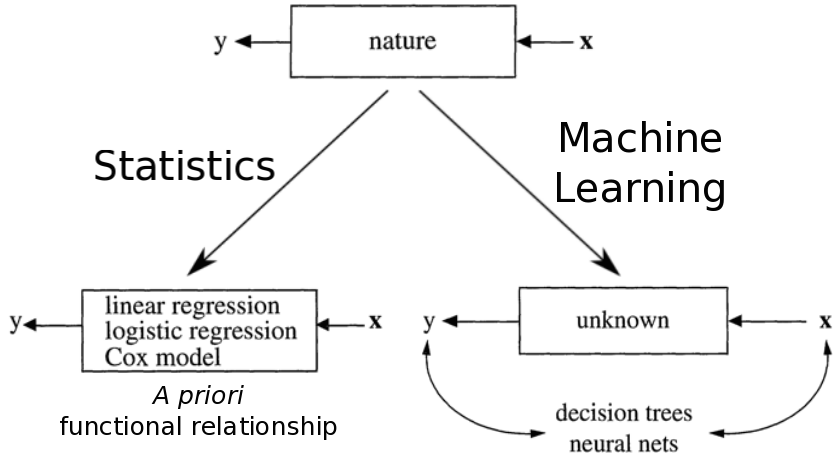
\includegraphics[width=0.85\textwidth]{statsvsML.png}
\end{center}
\end{frame}
%-------------------------------------------------------------------------------------------------%
\begin{frame}{Statistics vs Machine Learning}
\footnotesize %\small, \footnotesize, \scriptsize, \tiny
\begin{columns}
\column{0.49\textwidth}
\begin{block}{Statistics}
	\begin{itemize}\addtolength{\itemsep}{0.6\baselineskip}
		\item<2-> \textbf{Objective} - provide humans a set of data analysis tools 
		\item<3-> \textbf{Focus} - a probabilistic data model and its interpretability
		\item<4-> \textbf{Inference} - how was the observed data generated
		\item<5-> \textbf{Learning} - All measured data then perform inference on the population
		\item<6-> \textbf{Validation} - Measures of fit ($R^2$, chi-square test)
		\item<7-> \textbf{Selection} - Adjusted measures of fit (adjusted $R^2$, Cp statistic, AIC)
	\end{itemize}
\end{block}
\column{0.49\textwidth}	
\begin{block}{Machine Learning}
	\begin{itemize}\addtolength{\itemsep}{0.6\baselineskip}
		\item<2-> \textbf{Objective} - replace humans in the processing of data  
		\item<3-> \textbf{Focus} - algorithm that achieves excellent prediction accuracy
		\item<4-> \textbf{Prediction} - how can we use observed data to predict the future
		\item<5-> \textbf{Learning} - Training dataset then perform predictions on testing dataset
		\item<6-> \textbf{Validation} - How well it predicts ``unseen'' data (generalisation)
		\item<7-> \textbf{Selection} - Cross-validation and out-of-bag errors
	\end{itemize}
\end{block}
\end{columns}
\end{frame}
\normalsize
%-------------------------------------------------------------------------------------------------%
\begin{frame}{Statistics vs Machine Learning}
\begin{exampleblock}{}
{\small This enterprise (statistics) has at its heart the belief that a statistician, by imagination and by looking at the data, can invent a reasonably good parametric class of models for a complex mechanism devised by nature. Then parameters are estimated and conclusions are drawn. The conclusions are about the model's mechanism, and not about nature's mechanism!}
\vskip5mm
\hspace*\fill{\footnotesize --- Leo Breiman}
\end{exampleblock}
\vfill
\begin{exampleblock}{}
{\small The best solution could be an algorithmic model (machine learning), or maybe a data model, or maybe a combination. But the trick to being a scientist is to be open to using a wide variety of tools.}
\vskip5mm
\hspace*\fill{\footnotesize --- Leo Breiman}
\end{exampleblock}
\end{frame}
%-------------------------------------------------------------------------------------------------%
\begin{frame}{Formulating a machine learning problem}
\begin{enumerate}\addtolength{\itemsep}{0.5\baselineskip}
	\item<2-> Question/Hypothesis (start generic then narrow it down)
	\item<3-> Gather useful data
	\item<4-> \textbf{Extract features} (\textit{most important step})
	\item<5-> Choose a machine learning algorithm (\textit{probably least critical step})
	\item<6-> Build a predictive model
	\item<7-> Validate model
	\item<8-> Select model having the best generalisation capabilities
\end{enumerate}
\end{frame}
%-------------------------------------------------------------------------------------------------%
\begin{frame}{Terminology}
\begin{description}[Validation Dataset:]\addtolength{\itemsep}{0.5\baselineskip}
	\item<2->[Training Dataset:] Used to train a set of models
	\item<3->[Validation Dataset:] Used for model selection and validation. Helps us to select a 
	parsimonous model i.e a model which is complex enough to describe ``well'' our data but not more 
	complex
	\item<4->[Testing Dataset:] Used to compute the \textit{generalisation} error. Evaluate model
	performance on previously unseen data 
	\item<5->[Inputs:] Covariates, Predictors, Features, Attributes
	\item<6->[Training error:] In sample error, Resubstitution error
	\item<7->[Testing error:] Out of sample error, Generlisation error
\end{description}
\end{frame}
%-------------------------------------------------------------------------------------------------%
\begin{frame}{Applications in life sciences}
\begin{exampleblock}{Predicting fish species richness \vskip-1mm{\tiny Olden \textit{et al}. Q Rev Biol 2008, 83(2):171-193}}
\begin{description}
	\item[Features:] Lake surface area, shoreline perimeter, air temperature, precipitation and elevation
	% e.g mean = 5.3 --> average of 5.3 species for those particular conditions e.g area<=1.5km^2  
	\item[Method:] Decision trees (supervised)
\end{description}
\begin{center}
	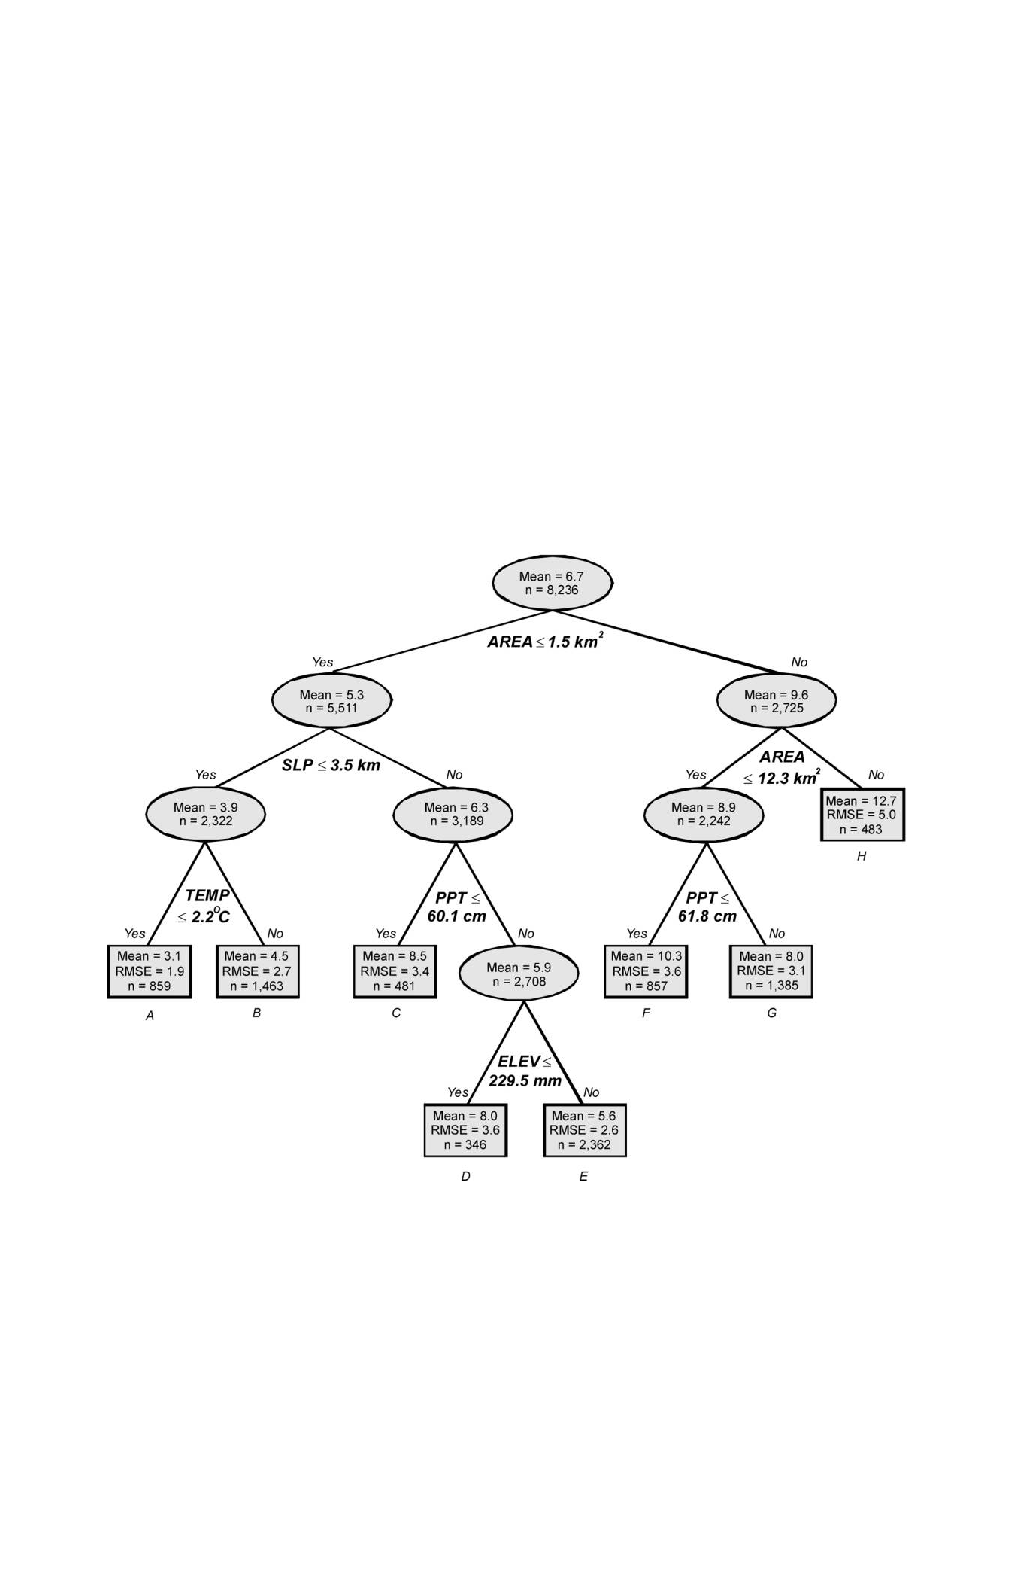
\includegraphics[width=0.5\textwidth]{olden.pdf}
\end{center}
\end{exampleblock}
\end{frame}
%-------------------------------------------------------------------------------------------------%
\begin{frame}{Applications in life sciences}
\begin{exampleblock}{Detection of malarial parasites \vskip-1mm{\tiny Purwar \textit{et al}. Malar J 2011, 10:364}}
\begin{description}
	\item[Features:] Image intensity
	\item[Method:] Modified k-means clustering (unsupervised)
\end{description}
\begin{center}
	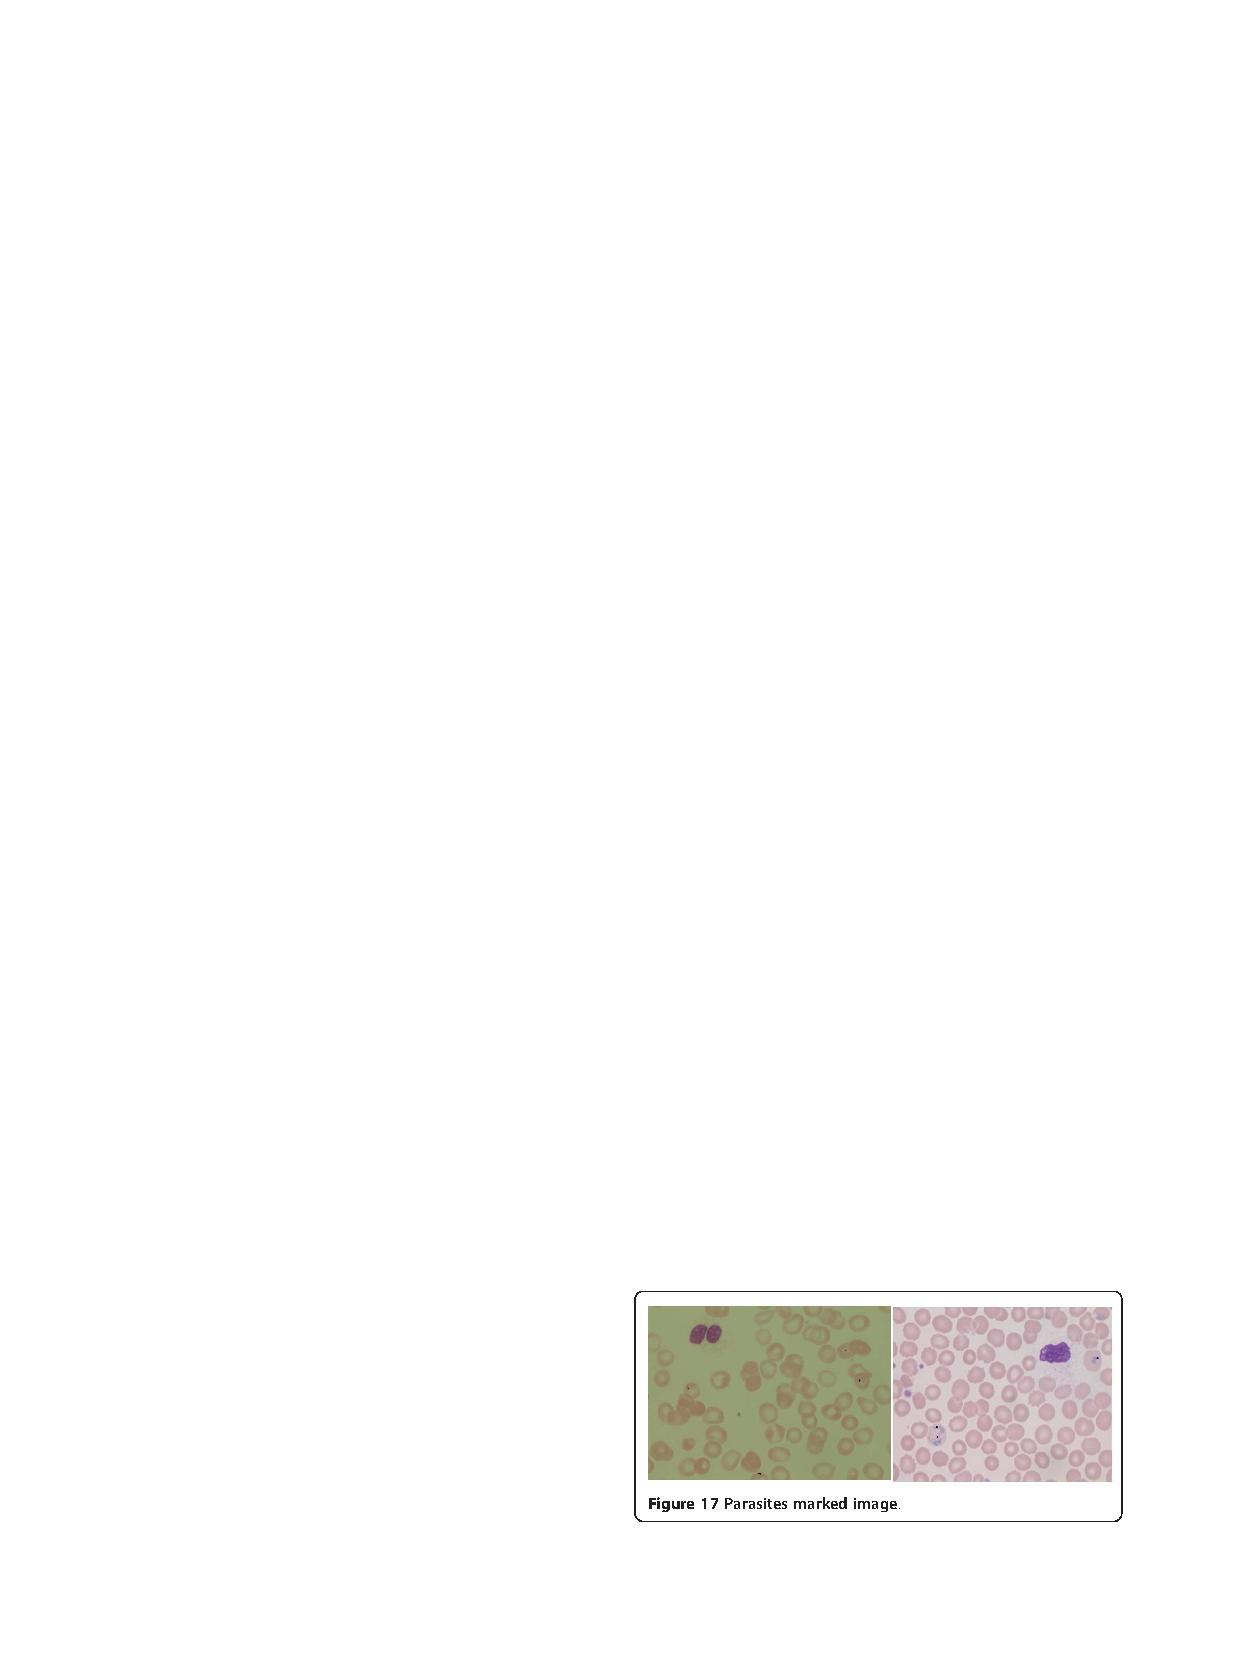
\includegraphics[width=0.54\textwidth]{purwar02.pdf}
	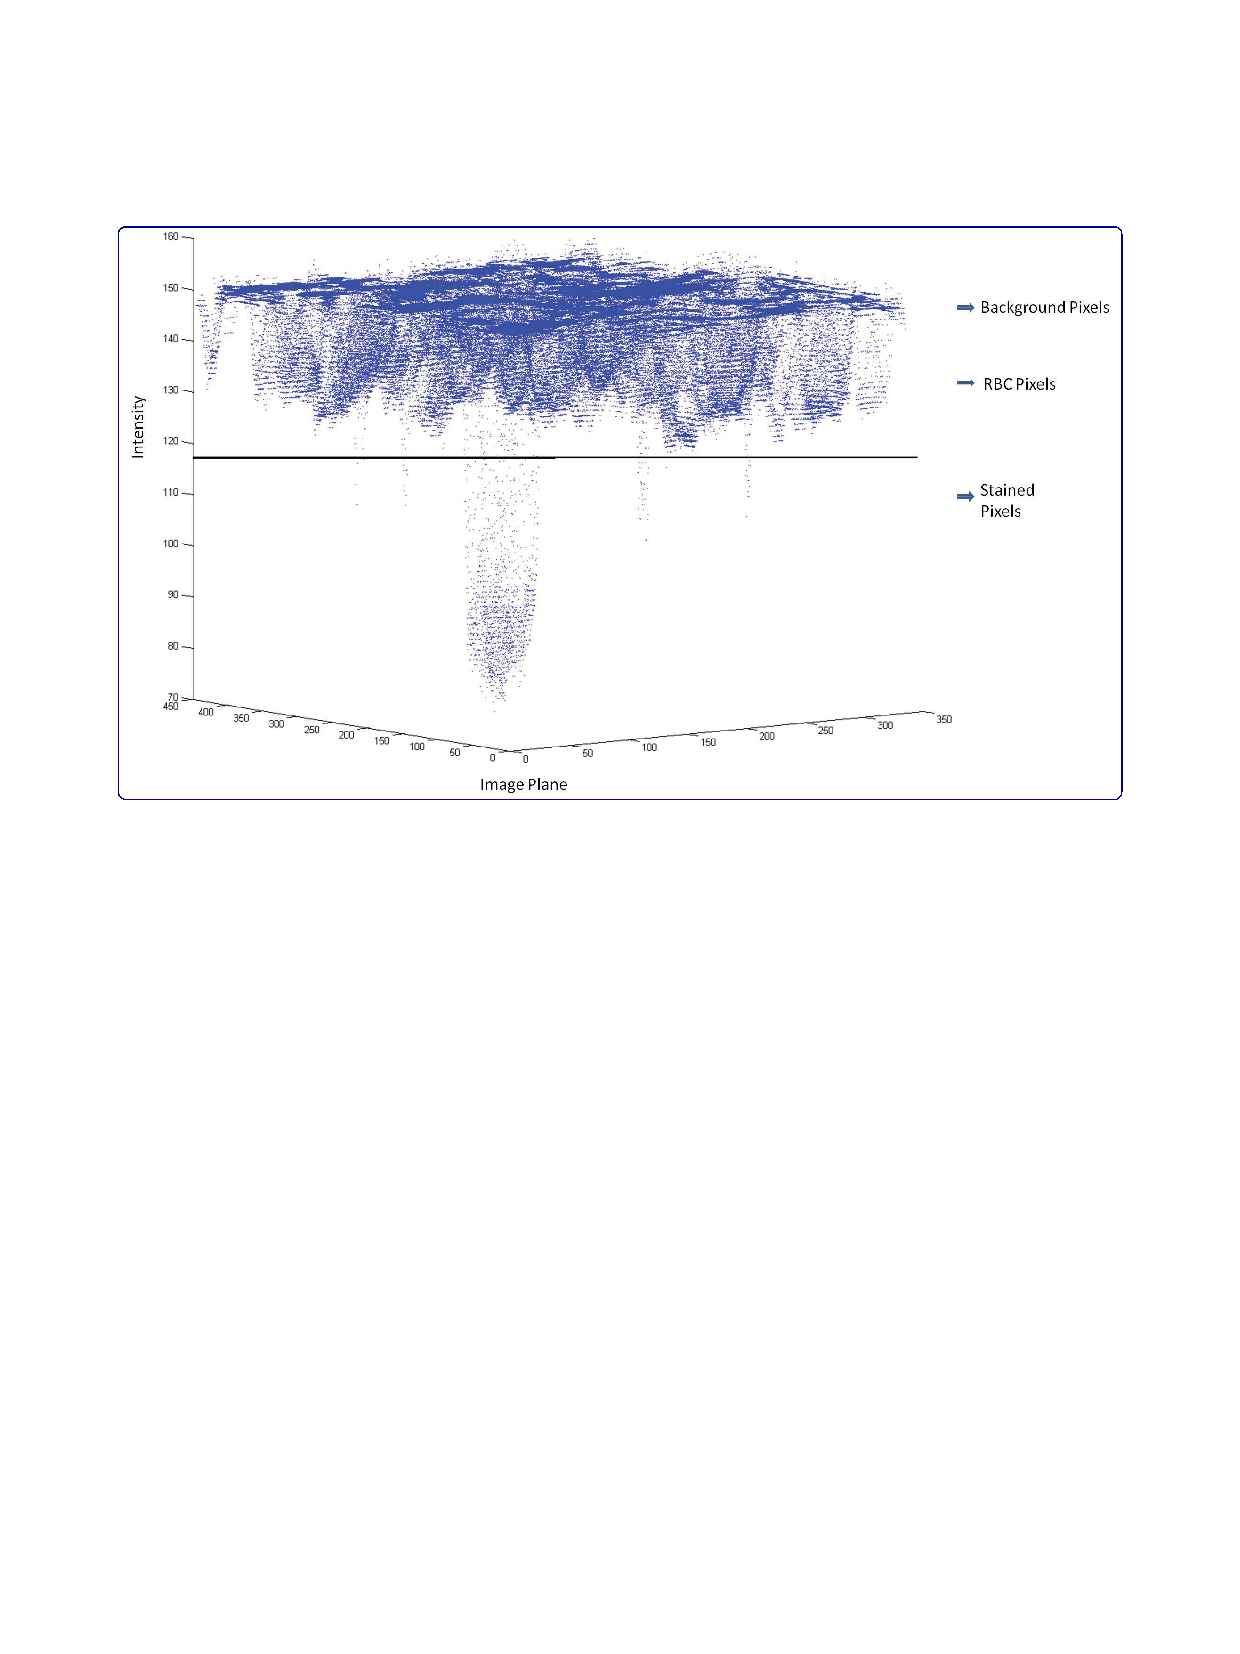
\includegraphics[width=0.46\textwidth]{purwar01.pdf}
\end{center}
\end{exampleblock}
\end{frame}
%-------------------------------------------------------------------------------------------------%
\begin{frame}{Applications in life sciences}
\begin{exampleblock}{Creating carbon-density maps \vskip-1mm{\tiny Baccini \textit{et al}. Nature Clim. Change 2012, 2:182-185}}
\begin{description}
	\item[Features:] Light detection and ranging (LiDAR) (elevation data)
	\item[Method:] Random forests (ensemble of decision trees) (supervised)
\end{description}
\begin{center}
	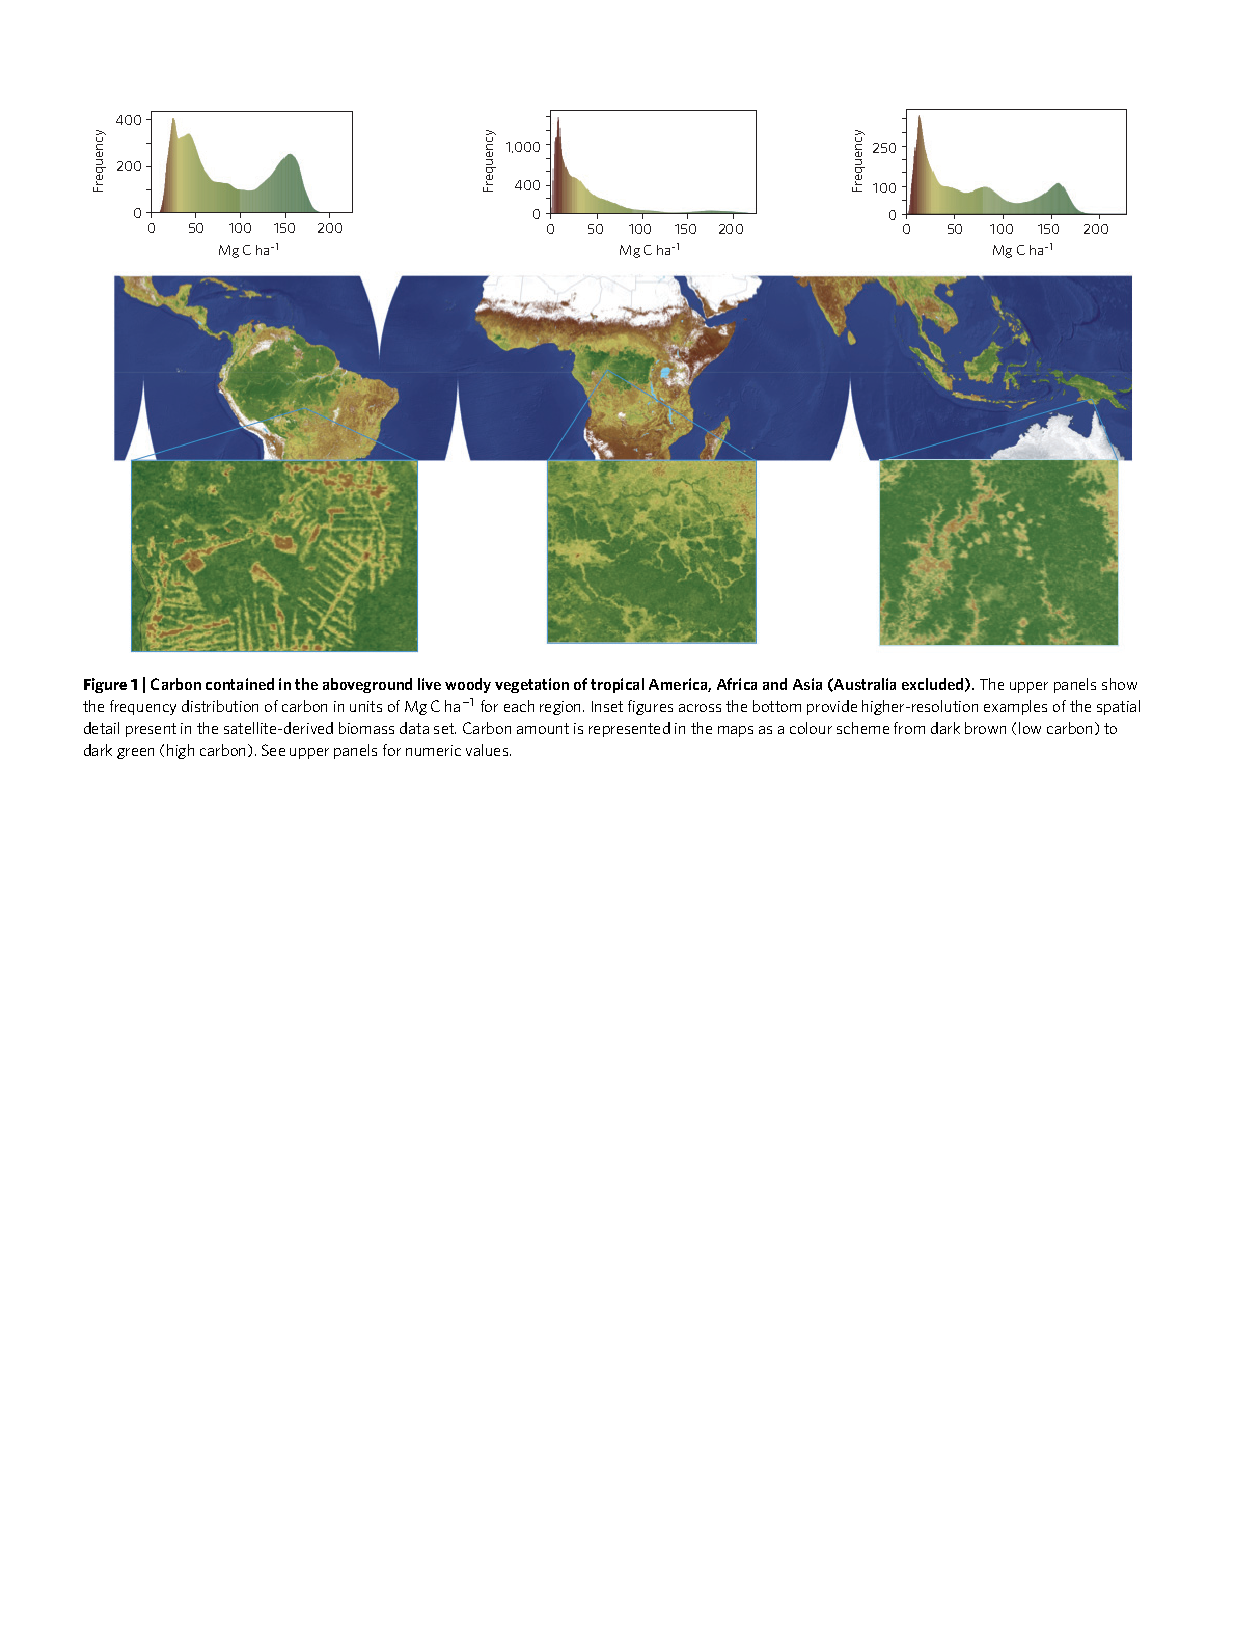
\includegraphics[width=0.74\textwidth]{baccini.pdf}
\end{center}
\end{exampleblock}
\end{frame}
%-------------------------------------------------------------------------------------------------%
\begin{frame}{Applications in life sciences}
\begin{exampleblock}{Acoustic classification of multiple simultaneous bird species \vskip-1mm{\tiny Briggs \textit{et al}. J Acoust Soc Am 2012, 131(6):4640-4650}}
\begin{description}
	\item[Features:] Segments in spectrogram (time vs frequency) from 10 secs audio recordings (corresponding to syllables of bird call)
	\item[Method:] Multi-instance multi-label learning (supervised)
\end{description}
\begin{center}
	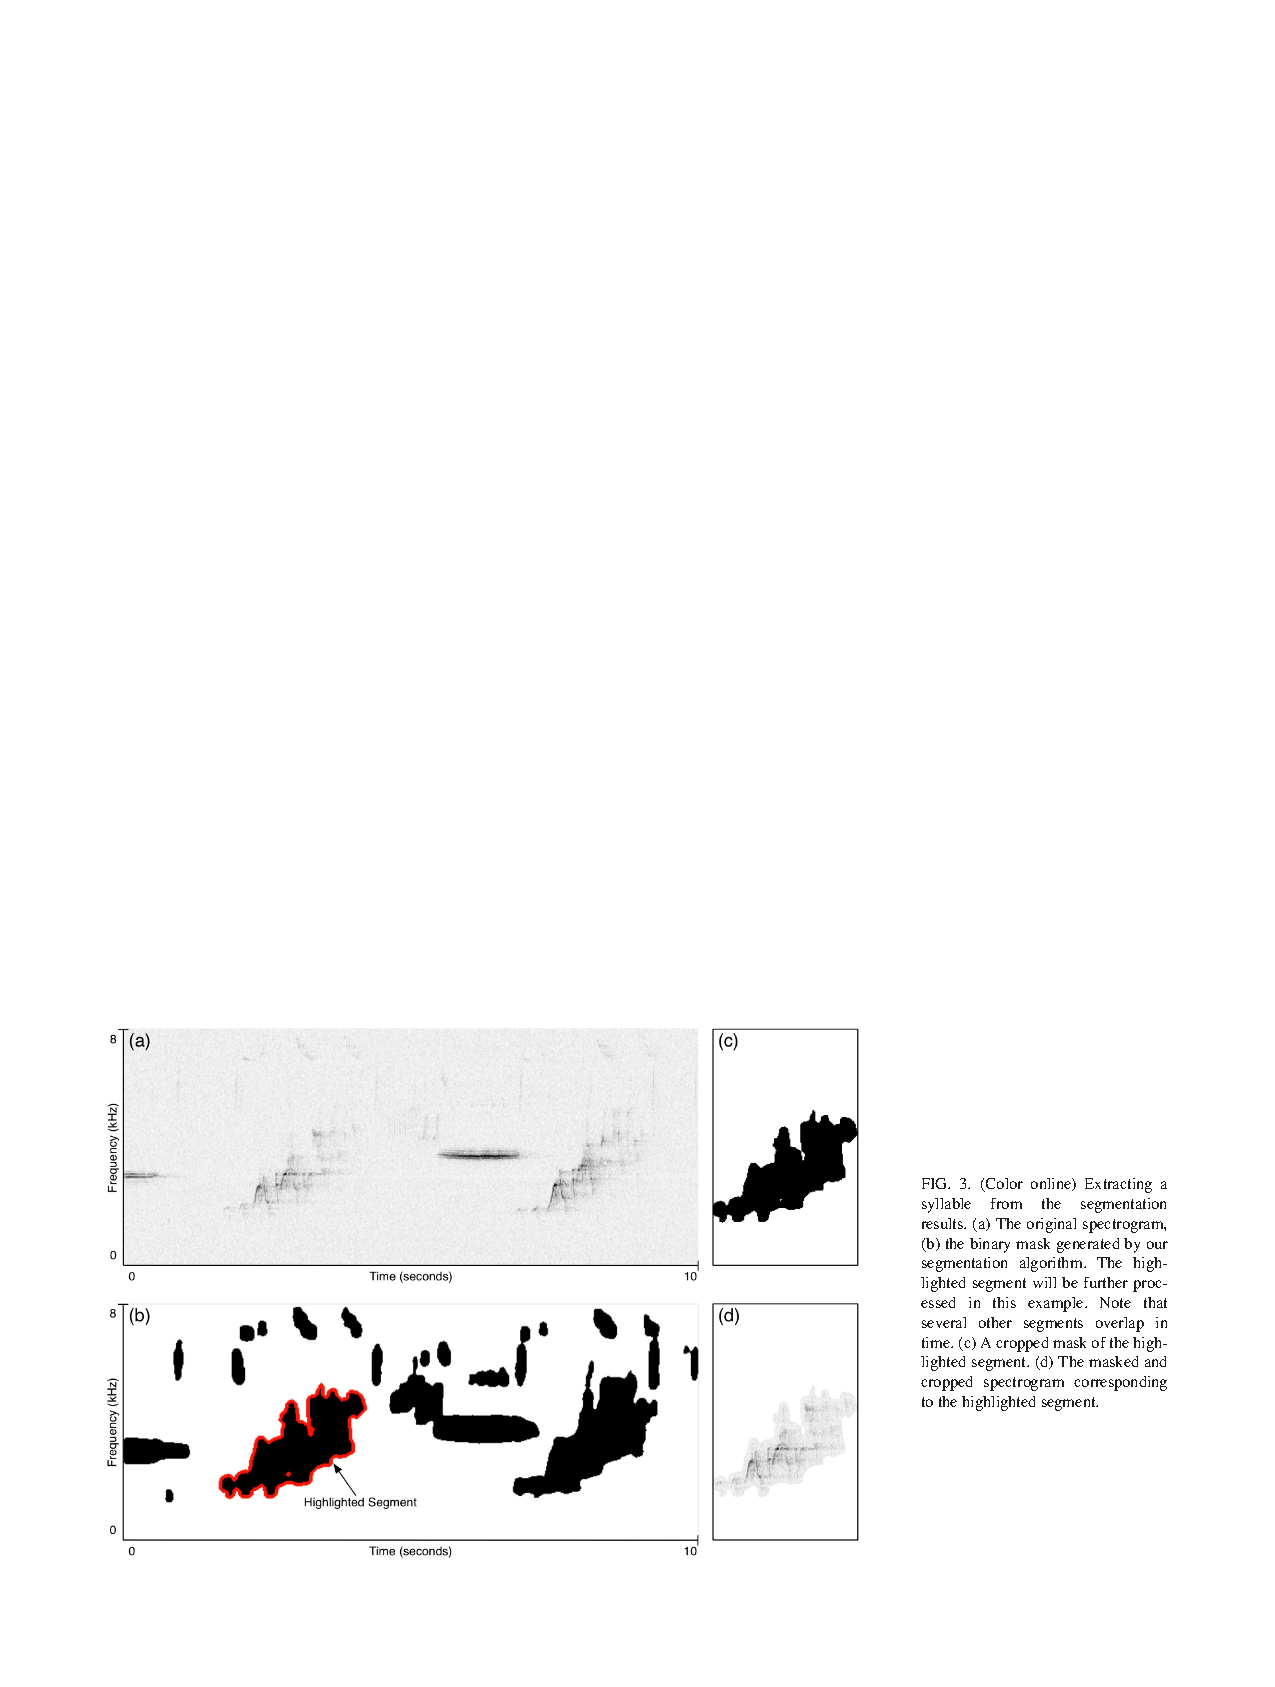
\includegraphics[width=0.8\textwidth]{briggs.pdf}
\end{center}
\end{exampleblock}
\end{frame}
%-------------------------------------------------------------------------------------------------%
\end{document}
%-------------------------------------------------------------------------------------------------%
% End of Document
%-------------------------------------------------------------------------------------------------%